\section{Dimensionamento del muro}
\subsection{Predimensionamento}
Il predimensionamento del muro avviene per via geometrica, secondo le misure indicate in \cref{figure:predimensionamento_muro}. Scelta un'altezza del muro H, si prosegue alla determinazione di primo tentativo di tutte le altre misure dell'opera.
\begin{figure}[H]
    \centering
    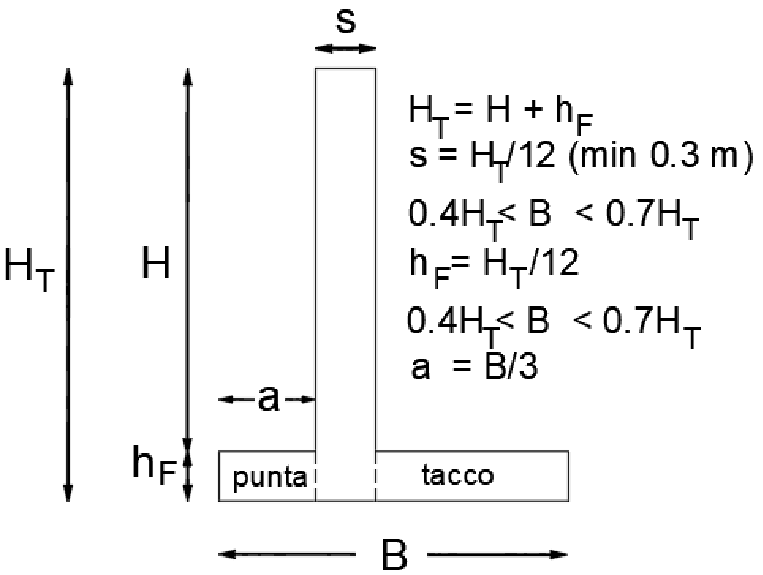
\includegraphics[width=0.5\textwidth]{immagini/predimensionamento_muro.pdf} \hfill
        \caption{Quote relative al predimensionamento (geometrico) del muro a mensola, secondo la normativa U.S.A. (U.S.A. Building Code).}
    \label{figure:predimensionamento_muro}
\end{figure}
Il tacco (t) e la punta (a) rappresentano le principali componenti geometriche della fondazione (B).

\subsection{Dimensionamento}
Partendo dalle dimensioni di massima dell'opera, ed utilizzando le diverse formule di verifica (che verranno esposte successivamente), in modo iterativo si è giunti al dimensionamento finale della struttura.

\begin{table}[H] \centering
\begin{tabular}{cccc}
    \toprule
Altezza muro & H & 3 m \\
Distanza lembo super. fondazione-piano campagna & $D_p$ & 0.4 \unit{m}  \\
Lunghezza muro & L & 10 \unit{m}  \\
Altezza fondazione & $H_f$ & 0.5 \unit{m}   \\
Altezza totale & $H_t$ & 3.5 \unit{m}   \\
Spessore muro & s & 0.5 \unit{m}  \\
Larghezza fondazione & B & 2.65 \unit{m}   \\
Tacco fondazione & t & 1.75 \unit{m}   \\
Punta fondazione & a & 0.4 \unit{m}   \\
\bottomrule
\end{tabular}
\end{table}

\subsection{Caratteristiche del terreno}
Il peso specifico del terreno asciutto($\gamma_D$) è funzione del peso specifico del terreno saturo ($\gamma_s$) e della sua porosità ($n$). La formula che lega queste tre caratteristiche è:
\begin{equation*}
    \gamma_d = \gamma_s \cdot (1-n)
\end{equation*} 
Essendo che l'angolo di resistenza al taglio del terreno è pari a $\phi$ = 33°, il coefficiente di spinta attiva $K_A$ è ricavato da:
\begin{equation*}
    K_A = tan^2 \left(45° - \frac{\phi}{2}\right) = tan^2 \left(45° - \frac{30}{2}\right) = 0.33
\end{equation*}